

\tikzset{every picture/.style={line width=0.75pt}} %set default line width to 0.75pt        

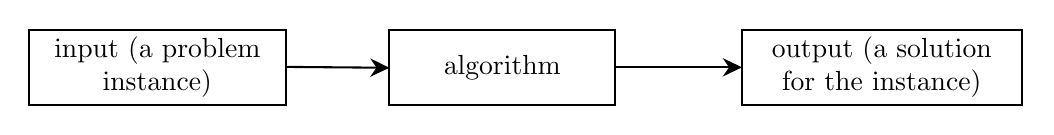
\begin{tikzpicture}[x=0.65pt,y=0.65pt,yscale=-1,xscale=1]
%uncomment if require: \path (0,173); %set diagram left start at 0, and has height of 173

%Shape: Rectangle [id:dp2688974996147625] 
\draw   (4.5,37.5) -- (147.5,37.5) -- (147.5,79.5) -- (4.5,79.5) -- cycle ;
%Shape: Rectangle [id:dp02749247312448544] 
\draw   (205,37.5) -- (330.5,37.5) -- (330.5,79.5) -- (205,79.5) -- cycle ;

%Shape: Rectangle [id:dp6309037575323136] 
\draw   (401,37.5) -- (556.5,37.5) -- (556.5,79.5) -- (401,79.5) -- cycle ;
%Straight Lines [id:da2596900380452606] 
\draw    (147.5,58.25) -- (202,58.72) ;
\draw [shift={(205,58.75)}, rotate = 180.5] [fill={rgb, 255:red, 0; green, 0; blue, 0 }  ][line width=0.08]  [draw opacity=0] (10.72,-5.15) -- (0,0) -- (10.72,5.15) -- (7.12,0) -- cycle    ;
%Straight Lines [id:da019692188199206262] 
\draw    (330.5,58.5) -- (398,58.5) ;
\draw [shift={(401,58.5)}, rotate = 180] [fill={rgb, 255:red, 0; green, 0; blue, 0 }  ][line width=0.08]  [draw opacity=0] (10.72,-5.15) -- (0,0) -- (10.72,5.15) -- (7.12,0) -- cycle    ;

% Text Node
\draw (267.75,58.5) node   [align=left] {algorithm};
% Text Node
\draw (76,58.5) node   [align=left] {\begin{minipage}[lt]{86.07pt}\setlength\topsep{0pt}
\begin{center}
input (a problem\\instance)
\end{center}

\end{minipage}};
% Text Node
\draw (478.75,58.5) node   [align=left] {\begin{minipage}[lt]{97.42pt}\setlength\topsep{0pt}
\begin{center}
output (a solution\\for the instance)
\end{center}

\end{minipage}};


\end{tikzpicture}
